\label{chp:Experiments}
..
\section{Data set}
\label{sec:Dataset}
The Wi-Fi CSI signature dataset~\cite{moon2017air} at position 1 was implemented in our experiment to mesure the performance of our proposed system. These are in-house Wi-Fi signature datasets that comprise 980 signatures per direction, as shown in~\ref{tab_dataset}. The size of each sample was 500 x 30 x 6. 
We utilized only the magnitues of the complex values, since the signal have device firmware issues in their phase information~\cite{wang2015understanding}. 
\begin{table}
    \caption{Description of the Dataset.}
    \label{tab_dataset}
    \begin{tabular}{ccc}
    \hline
    Direction of signature & \# of identities & \# of data \\ 
    \hline
    1                      & 98               & 980        \\ 
    2                      & 98               & 980        \\ 
    3                      & 98               & 980        \\ 
    4                      & 98               & 980        \\ 
    \hline
    \end{tabular}
\end{table}

\section{Experimental Settings}
This section details the evaluation scenarios and experimental settings.

\subsection{Evaluation Scenarios}
%performance
In this paper, the verification performance of the proposed method was evaluated in three ways:
I) In the first experiment, verification performance was compared between the proposed system and other systems including handcraft and deep-learning based methods.
II) Under the second experiments, Comparison of convergence speed was conducted between the proposed system other deep-learning based methods. 
III) The third experiments was conducted to compare the performance degradation between the proposed system and other deep-learning based methods when using a small sized feature vectors. 
In order to compare the feature extraction performance of the proposed system with other deep-learning based methods, we visualized feature space into 2d euclidean space by using PCA. 
% handcraft
We compared the proposed system both with handcraft methods and deep learning based methods.
For handcraft methods, least square estimations (LSE)~\cite{duda2012pattern}, the principal components analysis(PCA)~\cite{turk1991eigenfaces} with LSE, the supprot vector machine~\cite{vapnik2013nature} and the total error minimization with the reduced multivariate polynomal~\cite{toh2003fingerprint,toh2008between} were used. We selected parameters that perform optimally in each handcraft methods. For LSE,SVM and TER, the input signatures were reduced to 500$\times$30 by averaging the subcarrier Axis. For PCA-LSE, input signature dimension was reduced to 40 following~\cite{moon2017air}. For SVM with Gaussian kernel function (RBF), the kernel's parameters $c$ and $\gamma$ were chosen by a grid search over the range $c\in\{0.01,1,10\}$ and $\gamma\in\{0.01/3000, 0.1/3000, 1/3000, 10/3000, 100/3000\}$. For TER, parameter M is chosen among $M\in\{1,2,3\}$ and set $\tau=\eta=0.5$ following~\cite{toh2008between}.
For comparison with deep learning based methods, Siamese network~\cite{koch2015siamese} and baseline triplet network~\cite{hoffer2015deep} were used.
%protocols
The verification performance was evaluated in terms of the Equal Error Rate (EER, \%). We implemented a random 5-runs of 2-fold cross validation tests.
Due to the hardware memory limitations, we used downsized negative pairs according to the number of positive data pairs for calculating the EER. The size of positive data pairs and downsized negative pairs were 18620.

%5.2.2. Parameter settings
\subsection{Parameter Settings}
% KAR structure
For the proposed system, the structure of the KAR learning MLP sub-networks is shown in~\ref{kar_structure}. We empirically chosen two layers size of 1024 and 16. The size of the second layer was equivalent as feature vectors of the proposed ConvNet. The weights in the layers weree initialized as a normal distribution of 0 to 1 before training.
We used $tan^{-1}$ as an active function following~\cite{toh2018analytic}.
\begin{table}[]
    \caption{The network structure of KAR space learning.}
    \label{kar_structure}
    \centering
    \begin{tabular}{|l|l|l|}
    \hline
    Layer   & Size     & Activation \\ \hline
    Input   & 500$\times$30$\times$6 &            \\
    Fully-Connected 1 & 1$\times$1$\times$1024 & $\sigma = {tan}^{-1}$     \\
    Fully-Connected 2 & 1$\times$1$\times$16  & $\sigma = {tan}^{-1}$     \\
    Output  & 1$\times$1$\times$50   &            \\ \hline
    \end{tabular}
\end{table}
% conv structure
We used the same ConvNet structure shown in~\ref{conv_structure} and parameter settings for the proposed system and the deep-learning based methods. The CovNet structure consists of 3  convolution filters size of 3$\times$3 and stride 1. A ReLU activation function and 2$\times$2 max-pooling layers is applied between the filters. The depth of each layer was chosen as \{64,128,256\}. The output layer with sigmoid activation was regularized using $L2$ penalty of 0.0001. The size of the final feature vectors was 16.
\begin{table}[]
    \caption{The structure of ConvNet model.}
    \label{conv_structure}
    \centering
    \begin{tabular}{|c|c|c|c|}
    \hline
    Layer     & Activation & Kernel / Stride & Input Size \\ \hline
    Conv 1    & ReLU       & (3$\times$3)$\times$64/1      & 500$\times$30$\times$6   \\
    MaxPool 1 &            & (2$\times$2)/1         & 500$\times$30$\times$64  \\
    Conv 2    & ReLU       & (3$\times$3)$\times$128/1     & 250$\times$15$\times$64 \\
    MaxPool 2 &            & (2$\times$2)/1         & 250$\times$15$\times$128 \\
    Conv 3    & ReLU       & (3$\times$3)$\times$256/1     & 125$\times$8$\times$128  \\
    MaxPool 3 &            & (2$\times$2)/1         & 125$\times$8$\times$256  \\
    Fully-Connected     & Sigmoid    & 16             & 63$\times$4$\times$256   \\
    L-2 Norm  &            &                 & 1$\times$1$\times$16    \\
    Concat    &            &                 & 1$\times$1$\times$16    \\ \hline
    \end{tabular}
\end{table}
% traning parameters
The parameter settings for traning the deep learing network was 
learning rate of 0.0005, the number of iteration as 3000, and set the mini-batch size as 32. We used adam optimatizer for calculating the loss function. We initialized the ConvNet structures following ~\cite{koch2015siamese} before training. For convolution filters, we used a normal distribution of 0 mean and standard deviation of 0.0001. For the biases, parameters for normal distribution was 0.5 mean and standard deviation of 0.01. For calculating triplet loss, we set the alpha value as 0.5.

%5.3. Experimental results
\section{Experimental Results}
%5.3.1. verification performance
\subsection{Performance}
For experiment I,~\ref{tab_performance} shows the average EER from 5-runs of 2-fold cross-validation tests under the optimal parameter settings. As shown in Table~\ref{tab_performance}, the proposed system shows best performance among the handcraft and deep-learning based methods with 19.35\% EER.
Deep learning based methods performed better performance than handcraft methods since they were able to utilize the entire input signal, and their ability to feature extraction were better than handcraft methods.
\begin{table}[!h]
    \caption{Performance benchmarking with respect to the best EER (\%) averaged from five runs of two-fold cross-validation test on Wi-Fi CSI signature dataset.}\label{tab_performance}
    \centering
    \begin{tabular}{|c|c|c|}
    \hline
    Methology   &   Best EER (\%) &   Condition   \\  \hline
    LSE &   48.44   &  - \\ 
    PCA-LSE    &   30.79   &  Reduced dimension=40    \\
    SVM (Linear) &   28.23   &   c=1 \\
    SVM (RBF)    &   24.31   &   c=1, $\gamma$=0.01/3000 \\
    TER-RM2 &   35.84   &  M=1,$\tau$=$\eta$=0.5   \\     \hline
    Siamese network  &   23.53   &   lr=0.00005  \\
    Baseline triplet network &   20.34   &   lr=0.00005, $\alpha$=0.1  \\
    \textbf{Proposed system} &   \textbf{19.35}   &  \textbf{lr=0.00005, $\alpha$=0.1}  \\
     \hline
    \end{tabular}
\end{table}

%roc
As shown in~\ref{fig_roc}, the proposed system also showed the widest Area under ROC curve (AUC).
\begin{figure*}[!ht]
    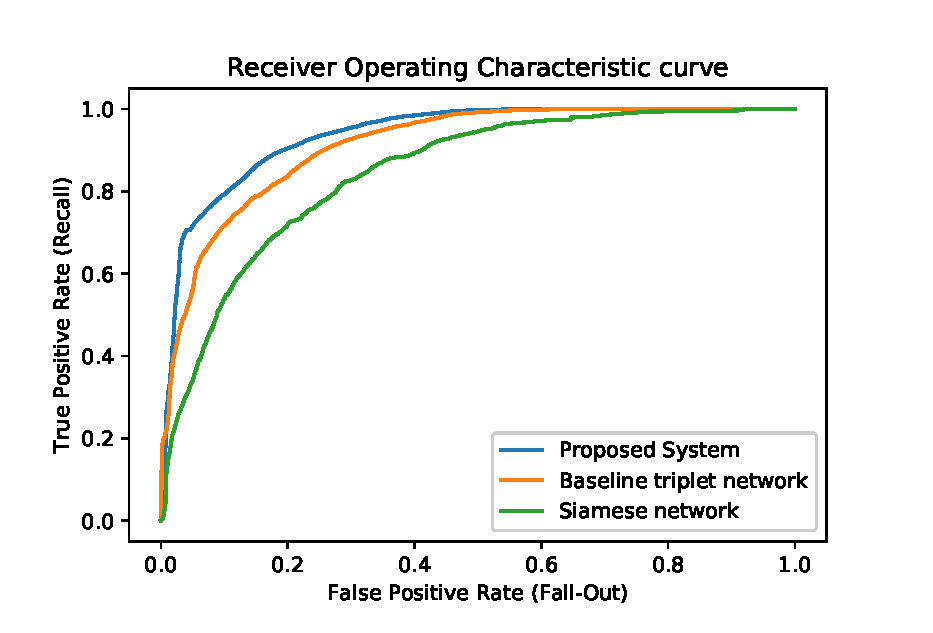
\includegraphics[width=\textwidth]{fig_roc_v15.eps}
    \caption{Normalized training loss curve.} \label{fig_roc}
\end{figure*}
 %5.3.1. conv speed
~\ref{fig_loss} shows the convergence of the normalized loss function during the training. The convergence speed of the proposed system was the fastest among the deep learning-based methods, meaning that KAR running has accelerated the learning speed.
\subsection{Convergence speed}
 \begin{figure*}[!ht]
    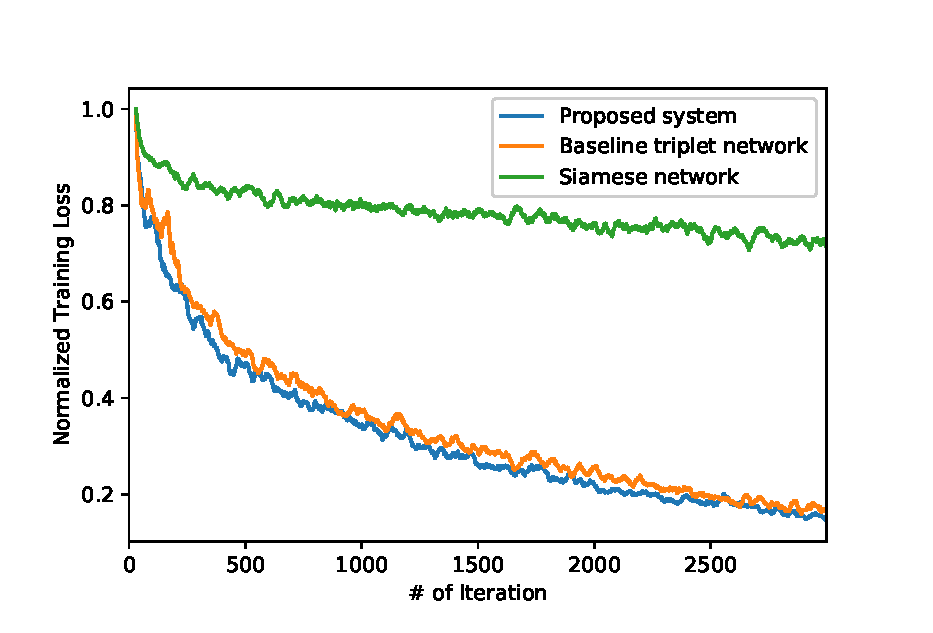
\includegraphics[width=\textwidth]{normalized_loss_curve_ma30_v3.eps}
    \caption{normalized training loss trends} \label{fig_loss}
\end{figure*}
%5.3.2. feature vector
\subsection{Effect of the size of Feature Vector}
- Case3) FC layer
○ Picture
○ The smaller the mapping to a characteristic space, the lower the performance degradation of the proposed method is.
§ Reason 1: Triplet network has better space placement capability than Siamese
Reason 2: Triplet network with KAR learning is better performance

\begin{table}[]
    \centering
    \begin{tabular}{|l|l|l|l|l|}
    \hline
    Size of the Feature Vector & 16    & 8     & 4     & 2     \\ \hline
    Siamese network            & 20.34 & 22.05 & 29.39 & 34.26 \\ \hline
    Baseline triplet network   & 18.37 & 19.52 & 19.20 & 24.76 \\ \hline
    Proposed system            & 16.92 & 18.03 & 18.08 & 26.64 \\ \hline
    \end{tabular}
\end{table}
\begin{figure}[!ht]
    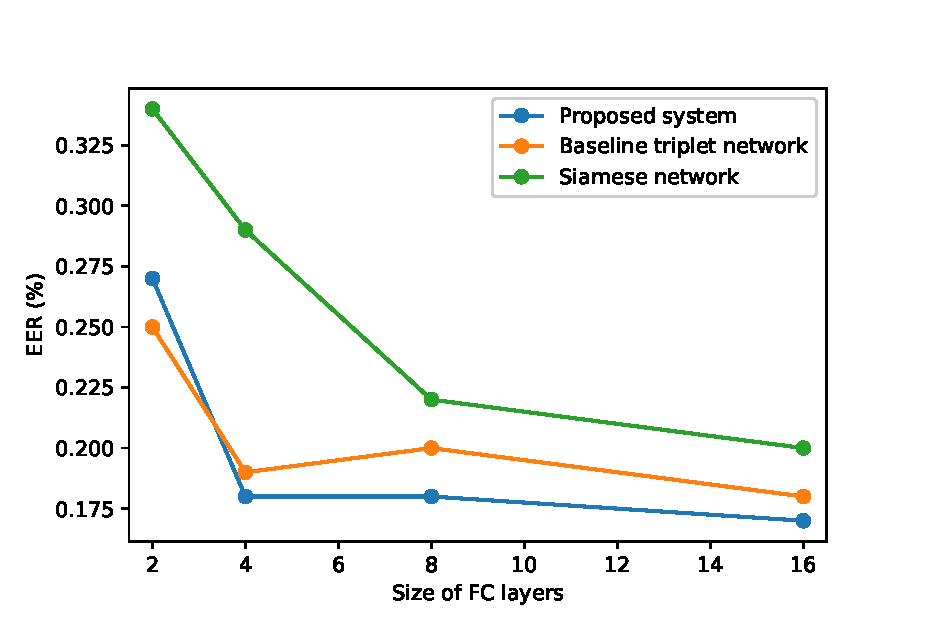
\includegraphics[width=\textwidth]{fclayer_v1.eps}
    \caption{Size of FC layer.} \label{fclayer}
\end{figure}

\begin{figure}[!ht]
    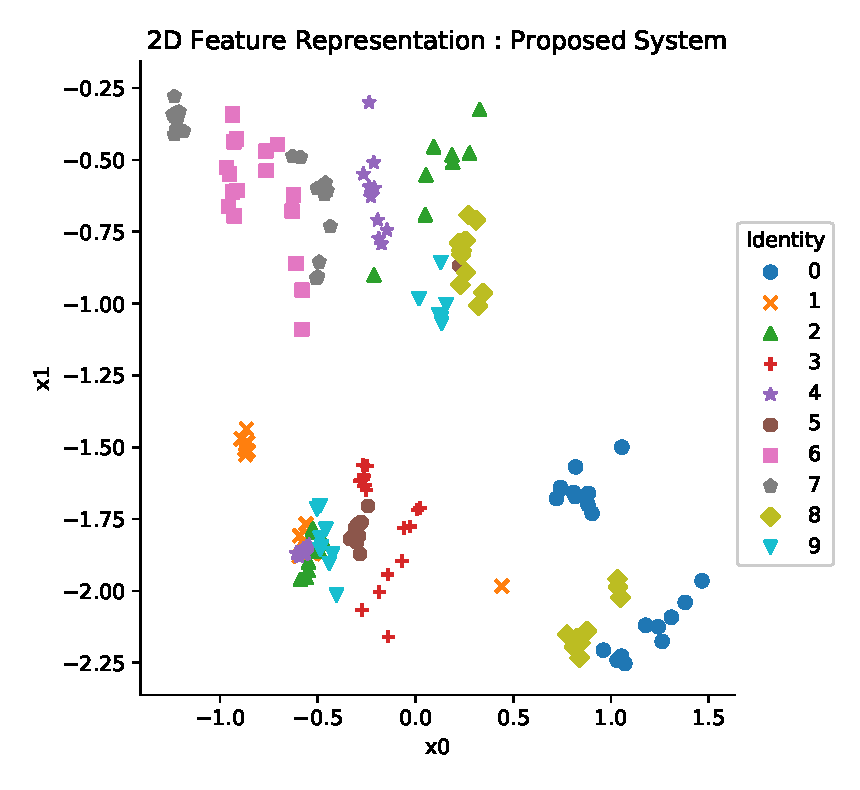
\includegraphics[width=\textwidth]{fig_2d_triKAR_10_v1.eps}
    \caption{2D Feature Representation : Proposed System.} \label{fig_2d_triKAR_10}
\end{figure}
\begin{figure}[!ht]
    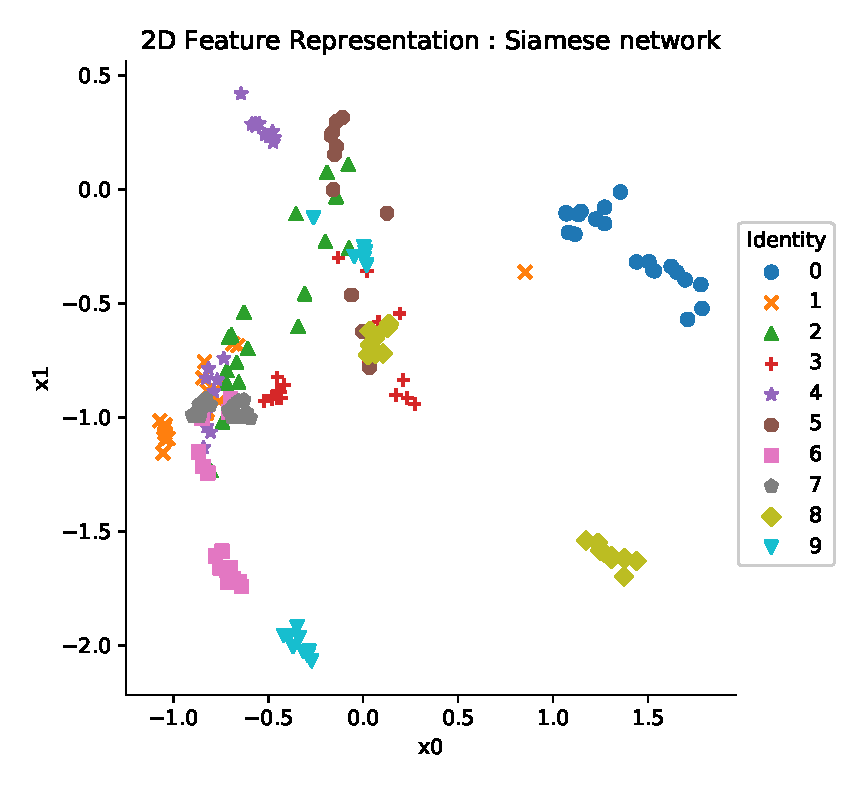
\includegraphics[width=\textwidth]{fig_2d_tribase_10_v1.eps}
    \caption{2D Feature Representation : Baseline triplet network.} \label{fig_2d_tribase_10}
\end{figure}
\begin{figure}[!ht]
    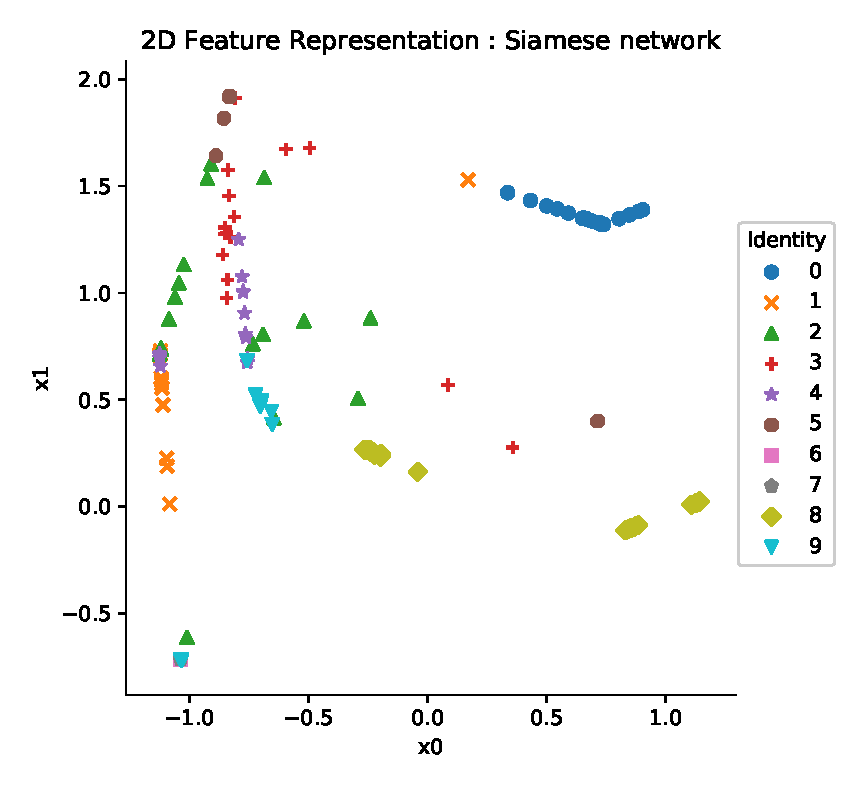
\includegraphics[width=\textwidth]{fig_2d_siam_10_v1.eps}
    \caption{2D Feature Representation : Siamese network.} \label{fig_2d_siam_10}
\end{figure}